

\chapter{The \bitstream Layer}

Conceptually, a \emph{bit stream}~$b$ is a sequence~$b_0,\ldots,b_{n-1}$ of $n$~bits.
Since the \isoc programming language does not allow to directly declare bit sequences
we represent bit streams as \emph{byte arrays}, that is, as arrays of type \inl{uint8_t}
(see Figure~\ref{fig:byte-array}).

\begin{figure}[hbt]
\begin{center}
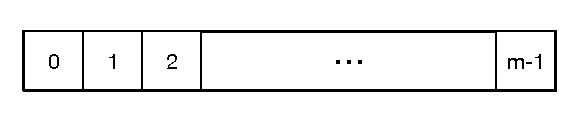
\includegraphics[scale=0.99]{Figures/byte-array.pdf}
\caption{Indexing in a byte array}
\label{fig:byte-array}
\end{center}
\end{figure}

If $x$ is a value of type \inl{uint8_t}, then its uniquely determined binary representation 
\begin{align*}
   x &= \sum_{i = 0}^{7} x_i\cdot 2^i && \text{with } x_k \in \{0, 1\} \text{ for } 0 \leq k < 8
\intertext{suggests an ordering of the bits of $x$ \emph{from the right}, that is, starting with the
position~0 of the \emph{least significant bit} of $x$}
   x &= (x_7,x_6,x_5,x_4,x_3,x_2,x_1,x_0)
\end{align*}

The ETCS standard, however, mandates that numerical values shall be transmitted
starting from the \emph{most significant bit}.
We therefore use the scheme of Figure~\ref{fig:bit-stream} for indexing bits within a byte stream.

\begin{figure}[hbt]
\begin{center}
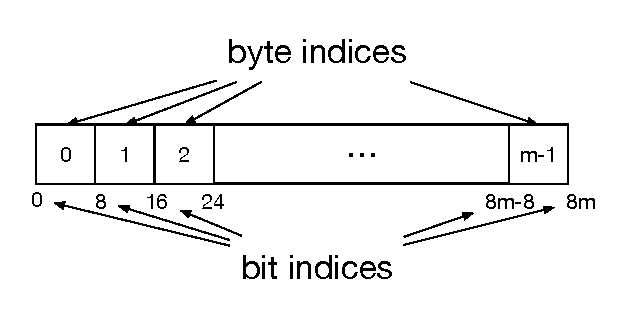
\includegraphics[scale=0.89]{Figures/bit-stream.pdf}
\caption{Indexing in a bit stream}
\label{fig:bit-stream}
\end{center}
\end{figure}

\section{The Type \bitstream and Related Functions}
\subsection{The Function \bitstreamread}
\subsection{The Function \inl{Bitstream_Write}}
\subsection{The Function \inl{NormalBitstream}}

\section{Predicates}
\subsection{\inl{Readable} and \inl{Writeable}}
\subsection{\inl{Invariant} and \inl{Normal}}
\subsection{\inl{EqualBits} and \inl{Unchanged}}
\subsection{\inl{UpperBitsNotSet}}

\section{Formal Specification}
\subsection{The Function \bitstreamread}
\subsection{The Function \inl{Bitstream_Write}}
\subsection{The Function \inl{NormalBitstream}}

\section{Implementation}
\subsection{The Function \bitstreamread}
\subsection{The Function \inl{Bitstream_Write}}
\subsection{The Function \inl{NormalBitstream}}

\section{Formal Verification}
\subsection{\inl{Bitstream_ReadThenWrite}}
\subsection{\inl{Bitstream_WriteThenRead}}

